\documentclass[11pt, oneside]{article}
\usepackage{geometry}
\geometry{letterpaper}
\usepackage{graphicx}
\usepackage{amssymb}
\usepackage{amsmath}
\usepackage{tikz}
\usepackage{tikz-qtree}
\usepackage{url}

\title{SICP Exercise 3.9}
\author{Yuchong Pan}

\begin{document}
\maketitle

The environment structure created by evaluating (factorial 6) using the recursive version of the \url{factorial} procedure is shown as follows:

\begin{center}
    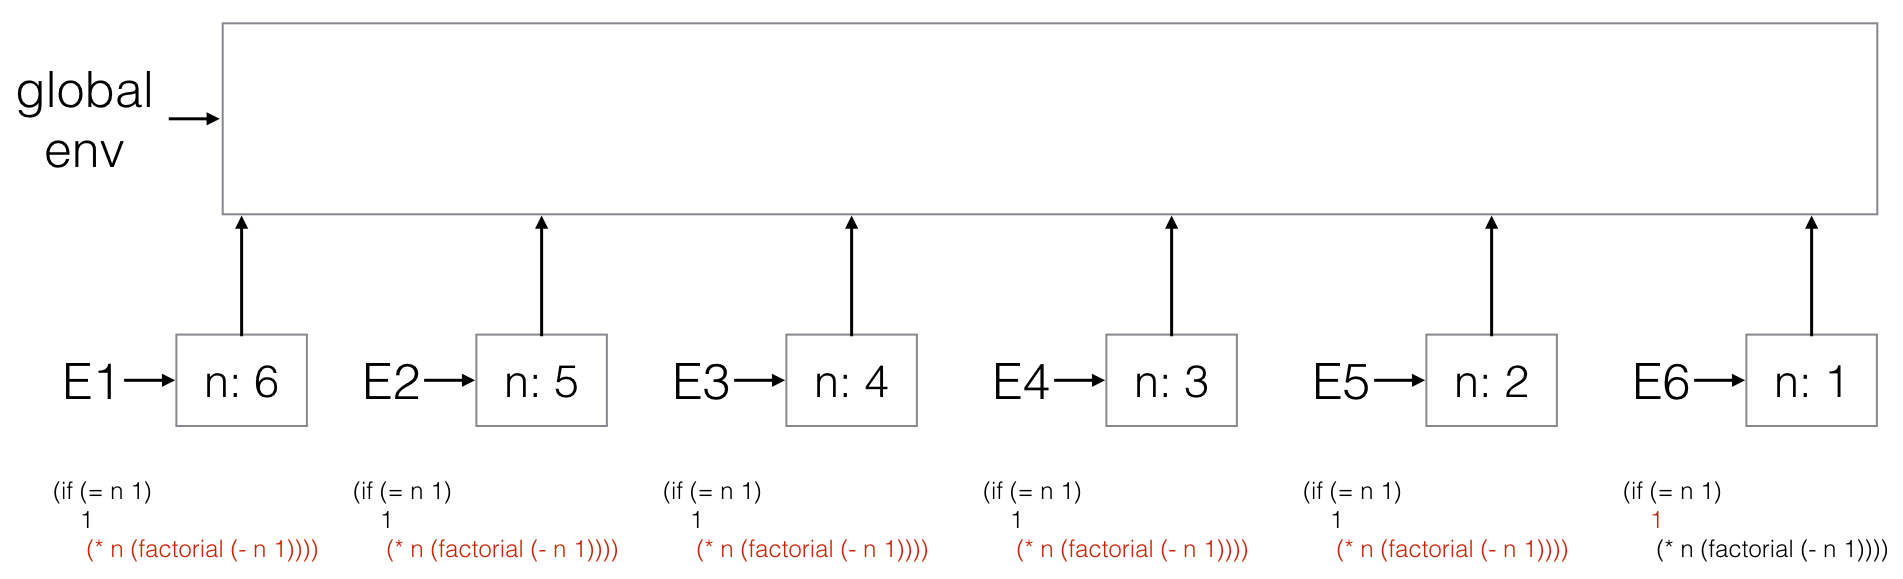
\includegraphics[width=15cm]{factorial-recursive.png}
\end{center}

The environment structure created by evaluating (factorial 6) using the iterative version of the \url{factorial} procedure is shown as follows:

\begin{center}
    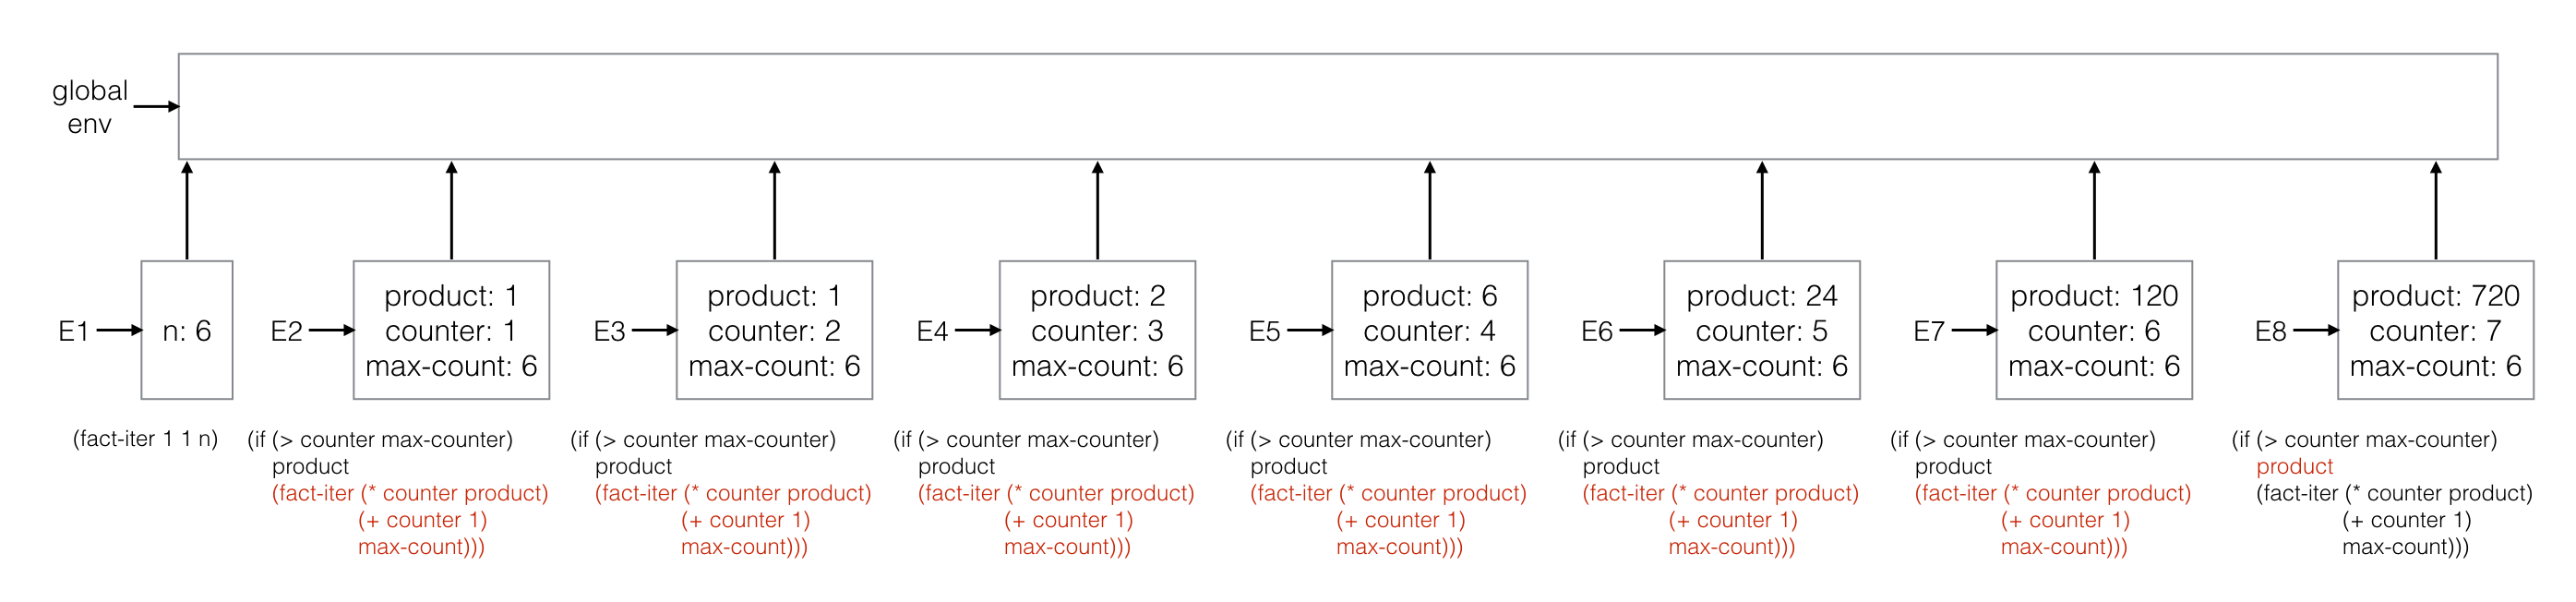
\includegraphics[width=15cm]{factorial-iterative.png}
\end{center}

\end{document}
